\documentclass[border=4pt]{standalone}
\usepackage{tikz}
\usetikzlibrary{arrows.meta, calc, decorations.markings}
\usepackage{amsmath}

\definecolor{traitor}{HTML}{b2182b}
\definecolor{faithful}{HTML}{2166ac}
\definecolor{dead}{HTML}{cccccc}
\definecolor{accent}{HTML}{1b7837}
\definecolor{warn}{HTML}{e08214}
\definecolor{panelbg}{HTML}{fafafa}

\begin{document}
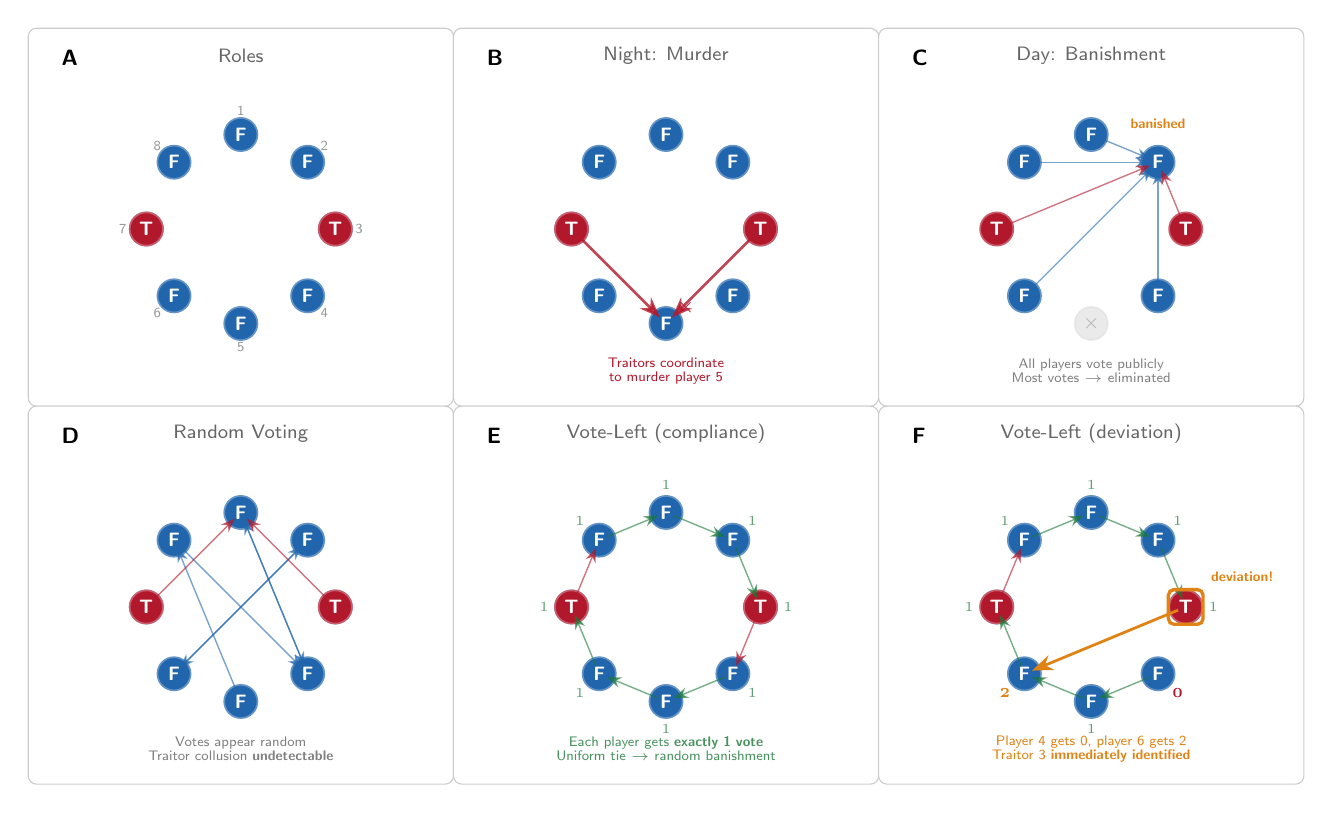
\begin{tikzpicture}[
    >=Stealth,
    font=\sffamily,
    player/.style={circle, minimum size=12pt, inner sep=0pt, line width=0.6pt,
                   font=\sffamily\scriptsize\bfseries, text=white},
    fnode/.style={player, fill=faithful, draw=faithful!70},
    tnode/.style={player, fill=traitor, draw=traitor!70},
    dnode/.style={player, fill=dead, draw=dead!80, opacity=0.4,
                  font=\sffamily\scriptsize\bfseries, text=black!60},
    votearrow/.style={->, line width=0.5pt, opacity=0.6},
    killarrow/.style={->, line width=1.0pt, traitor, opacity=0.8},
    panellabel/.style={font=\sffamily\footnotesize\bfseries, anchor=north west},
    caption/.style={font=\sffamily\scriptsize, text=black!60, align=center},
]

% ── Layout: 2 rows x 3 cols, each panel ~4.2cm wide ──
\def\pw{4.8}   % panel width
\def\ph{4.2}   % panel height
\def\gap{0.6}  % gap between panels
\def\R{1.2}    % circle radius for players

% Panel origins (bottom-left of each)
\coordinate (P1) at (0, \ph+\gap);
\coordinate (P2) at (\pw+\gap, \ph+\gap);
\coordinate (P3) at (2*\pw+2*\gap, \ph+\gap);
\coordinate (P4) at (0, 0);
\coordinate (P5) at (\pw+\gap, 0);
\coordinate (P6) at (2*\pw+2*\gap, 0);

% ── Helper: draw 8 players in a circle ──
% Args: center, prefix, traitor list (1-indexed)
\newcommand{\drawplayers}[3]{
    % #1 = center, #2 = prefix, #3 = comma-separated traitor positions
    \foreach \i in {1,...,8} {
        \pgfmathsetmacro{\angle}{90 - (\i-1)*45}
        \coordinate (#2-\i) at ($(#1) + (\angle:\R)$);
    }
    % Draw faithful first (F label), then traitors on top (T label)
    \foreach \i in {1,...,8} {
        \node[fnode] at (#2-\i) {F};
    }
    \foreach \t in {#3} {
        \node[tnode] at (#2-\t) {T};
    }
}

% ══════════════════════════════════════════════════════════════
% TOP ROW: Game phases
% ══════════════════════════════════════════════════════════════

% ── Panel A: Roles ──
\begin{scope}[shift=(P1)]
    \draw[draw=black!20, fill=white, rounded corners=3pt] (-0.3, -0.3) rectangle (\pw+0.3, \ph+0.3);
    \node[panellabel] at (0, \ph+0.15) {A};
    \node[caption] at (\pw/2, \ph-0.05) {Roles};

    \pgfmathsetmacro{\cx}{\pw/2}
    \pgfmathsetmacro{\cy}{\ph/2 - 0.15}
    \coordinate (CA) at (\cx, \cy);
    \drawplayers{CA}{a}{3,7}

    % % Legend
    % \node[fnode, minimum size=10pt] at (3.35, 0.6) {F};
    % \node[font=\sffamily\tiny, text=faithful, anchor=west] at (3.55, 0.6) {Faithful};
    % \node[tnode, minimum size=10pt] at (3.35, 0.25) {T};
    % \node[font=\sffamily\tiny, text=traitor, anchor=west] at (3.55, 0.25) {Traitor};

    % Player numbers
    \foreach \i in {1,...,8} {
        \pgfmathsetmacro{\angle}{90 - (\i-1)*45}
        \node[font=\sffamily\tiny, text=black!40] at ($(CA) + (\angle:\R+0.3)$) {\i};
    }
\end{scope}

% ── Panel B: Night (Murder) ──
\begin{scope}[shift=(P2)]
    \draw[draw=black!20, fill=white, rounded corners=3pt] (-0.3, -0.3) rectangle (\pw+0.3, \ph+0.3);
    \node[panellabel] at (0, \ph+0.15) {B};
    \node[caption] at (\pw/2, \ph-0.05) {Night: Murder};

    \pgfmathsetmacro{\cx}{\pw/2}
    \pgfmathsetmacro{\cy}{\ph/2 - 0.15}
    \coordinate (CB) at (\cx, \cy);
    \drawplayers{CB}{b}{3,7}

    % Murder arrow: traitors 3 and 7 target faithful 5
    \draw[killarrow, shorten >=3pt, shorten <=3pt] (b-3) -- (b-5);
    \draw[killarrow, shorten >=3pt, shorten <=3pt] (b-7) -- (b-5);

    % X on victim
    \node[font=\sffamily\scriptsize\bfseries, text=traitor] at ($(b-5)+(0.25, 0.2)$) {$\times$};

    % Annotation
    \node[font=\sffamily\tiny, text=traitor, align=center] at (\pw/2, 0.15) {Traitors coordinate\\[-1pt]to murder player 5};
\end{scope}

% ── Panel C: Day (Banishment) ──
\begin{scope}[shift=(P3)]
    \draw[draw=black!20, fill=white, rounded corners=3pt] (-0.3, -0.3) rectangle (\pw+0.3, \ph+0.3);
    \node[panellabel] at (0, \ph+0.15) {C};
    \node[caption] at (\pw/2, \ph-0.05) {Day: Banishment};

    \pgfmathsetmacro{\cx}{\pw/2}
    \pgfmathsetmacro{\cy}{\ph/2 - 0.15}
    \coordinate (CC) at (\cx, \cy);

    % Player 5 is dead
    \foreach \i in {1,...,8} {
        \pgfmathsetmacro{\angle}{90 - (\i-1)*45}
        \coordinate (c-\i) at ($(CC) + (\angle:\R)$);
    }
    \foreach \i in {1,2,4,6,8} {
        \node[fnode] at (c-\i) {F};
    }
    \node[tnode] at (c-3) {T};
    \node[tnode] at (c-7) {T};
    \node[dnode] at (c-5) {$\times$};

    % Show some votes converging on player 2 (banished)
    \foreach \src in {1,4,6,8} {
        \draw[votearrow, faithful, shorten >=3pt, shorten <=3pt] (c-\src) -- (c-2);
    }
    \draw[votearrow, traitor, shorten >=3pt, shorten <=3pt] (c-3) -- (c-2);
    \draw[votearrow, traitor, shorten >=3pt, shorten <=3pt] (c-7) -- (c-2);

    % Banished marker
    \node[font=\sffamily\tiny\bfseries, text=warn, anchor=south] at ($(c-2)+(0, 0.3)$) {banished};

    \node[font=\sffamily\tiny, text=black!50, align=center] at (\pw/2, 0.15) {All players vote publicly\\[-1pt]Most votes $\to$ eliminated};
\end{scope}

% ══════════════════════════════════════════════════════════════
% BOTTOM ROW: Voting strategies
% ══════════════════════════════════════════════════════════════

% ── Panel D: Random Voting ──
\begin{scope}[shift=(P4)]
    \draw[draw=black!20, fill=white, rounded corners=3pt] (-0.3, -0.3) rectangle (\pw+0.3, \ph+0.3);
    \node[panellabel] at (0, \ph+0.15) {D};
    \node[caption] at (\pw/2, \ph-0.05) {Random Voting};

    \pgfmathsetmacro{\cx}{\pw/2}
    \pgfmathsetmacro{\cy}{\ph/2 - 0.15}
    \coordinate (CD) at (\cx, \cy);
    \drawplayers{CD}{d}{3,7}

    % Random scattered votes (each to a different target)
    \draw[votearrow, faithful, shorten >=3pt, shorten <=3pt] (d-1) -- (d-4);
    \draw[votearrow, faithful, shorten >=3pt, shorten <=3pt] (d-2) -- (d-6);
    \draw[votearrow, faithful, shorten >=3pt, shorten <=3pt] (d-4) -- (d-1);
    \draw[votearrow, faithful, shorten >=3pt, shorten <=3pt] (d-5) -- (d-8);
    \draw[votearrow, faithful, shorten >=3pt, shorten <=3pt] (d-6) -- (d-2);
    \draw[votearrow, faithful, shorten >=3pt, shorten <=3pt] (d-8) -- (d-4);
    % Traitors collude: both vote for player 1
    \draw[votearrow, traitor, shorten >=3pt, shorten <=3pt] (d-3) -- (d-1);
    \draw[votearrow, traitor, shorten >=3pt, shorten <=3pt] (d-7) -- (d-1);

    \node[font=\sffamily\tiny, text=black!50, align=center] at (\pw/2, 0.15) {Votes appear random\\[-1pt]Traitor collusion \textbf{undetectable}};
\end{scope}

% ── Panel E: Vote-Left (compliance) ──
\begin{scope}[shift=(P5)]
    \draw[draw=black!20, fill=white, rounded corners=3pt] (-0.3, -0.3) rectangle (\pw+0.3, \ph+0.3);
    \node[panellabel] at (0, \ph+0.15) {E};
    \node[caption] at (\pw/2, \ph-0.05) {Vote-Left (compliance)};

    \pgfmathsetmacro{\cx}{\pw/2}
    \pgfmathsetmacro{\cy}{\ph/2 - 0.15}
    \coordinate (CE) at (\cx, \cy);
    \drawplayers{CE}{e}{3,7}

    % Each player votes for the next clockwise (1→2, 2→3, ..., 8→1)
    \foreach \i [evaluate=\i as \j using {int(mod(\i, 8) + 1)}] in {1,...,8} {
        \pgfmathsetmacro{\isTraitor}{\i == 3 || \i == 7 ? 1 : 0}
        \ifnum\isTraitor=1
            \draw[votearrow, traitor, shorten >=3pt, shorten <=3pt] (e-\i) -- (e-\j);
        \else
            \draw[votearrow, accent, shorten >=3pt, shorten <=3pt] (e-\i) -- (e-\j);
        \fi
    }

    % Tick marks: everyone gets 1 vote
    \foreach \i in {1,...,8} {
        \pgfmathsetmacro{\angle}{90 - (\i-1)*45}
        \node[font=\tiny, text=accent!70] at ($(CE) + (\angle:\R+0.35)$) {1};
    }

    \node[font=\sffamily\tiny, text=accent!80, align=center] at (\pw/2, 0.15) {Each player gets \textbf{exactly 1 vote}\\[-1pt]Uniform tie $\to$ random banishment};
\end{scope}

% ── Panel F: Vote-Left (deviation detected) ──
\begin{scope}[shift=(P6)]
    \draw[draw=black!20, fill=white, rounded corners=3pt] (-0.3, -0.3) rectangle (\pw+0.3, \ph+0.3);
    \node[panellabel] at (0, \ph+0.15) {F};
    \node[caption] at (\pw/2, \ph-0.05) {Vote-Left (deviation)};

    \pgfmathsetmacro{\cx}{\pw/2}
    \pgfmathsetmacro{\cy}{\ph/2 - 0.15}
    \coordinate (CF) at (\cx, \cy);
    \drawplayers{CF}{f}{3,7}

    % Faithful comply: vote for next
    \foreach \i [evaluate=\i as \j using {int(mod(\i, 8) + 1)}] in {1,2,4,5,6,8} {
        \draw[votearrow, accent, shorten >=3pt, shorten <=3pt] (f-\i) -- (f-\j);
    }

    % Traitor 7 complies (votes for 8)
    \draw[votearrow, traitor, shorten >=3pt, shorten <=3pt] (f-7) -- (f-8);

    % Traitor 3 DEVIATES: votes for player 6 instead of 4
    \draw[->, line width=1.0pt, warn, shorten >=3pt, shorten <=3pt] (f-3) -- (f-6);

    % Highlight the deviation
    \draw[warn, line width=1.2pt, rounded corners=2pt]
        ($(f-3)+(-0.22,-0.22)$) rectangle ($(f-3)+(0.22,0.22)$);
    \node[font=\sffamily\tiny\bfseries, text=warn, anchor=south west] at ($(f-3)+(0.2, 0.2)$) {deviation!};

    % Vote counts showing the break. Player i sits at angle 90-(i-1)*45:
    % 1=90, 2=45, 3=0, 4=-45, 5=-90, 6=-135, 7=180, 8=135.
    \node[font=\tiny, text=accent!70] at ($(CF) + (90:\R+0.35)$) {1};    % player 1
    \node[font=\tiny, text=accent!70] at ($(CF) + (45:\R+0.35)$) {1};    % player 2
    \node[font=\tiny, text=accent!70] at ($(CF) + (0:\R+0.35)$) {1};     % player 3
    % player 4 gets 0 votes (traitor 3 deviated away from them)
    \node[font=\tiny\bfseries, text=traitor] at ($(CF) + (-45:\R+0.35)$) {0};
    \node[font=\tiny, text=accent!70] at ($(CF) + (-90:\R+0.35)$) {1};   % player 5
    % player 6 gets 2 votes (from player 5 and from the deviating traitor 3)
    \node[font=\tiny\bfseries, text=warn] at ($(CF) + (-135:\R+0.35)$) {2};
    \node[font=\tiny, text=accent!70] at ($(CF) + (180:\R+0.35)$) {1};   % player 7
    \node[font=\tiny, text=accent!70] at ($(CF) + (135:\R+0.35)$) {1};   % player 8

    \node[font=\sffamily\tiny, text=warn, align=center] at (\pw/2, 0.15) {Player 4 gets 0, player 6 gets 2\\[-1pt]Traitor 3 \textbf{immediately identified}};
\end{scope}

\end{tikzpicture}
\end{document}
